\documentclass{article}
\usepackage[utf8]{inputenc}
\usepackage{graphicx}

\title{Primeira fase do projeto de MAC0350}
\author{Gustavo Silva - 9298260\\Leonardo Padilha - 9298295 \\Lucas Santos - 9345064 \\Marcos Kawakami - 8041331 \\Matheus Oliveira - 8642821 \\Victor Sena Molero - 8941317}
\date{}

\begin{document}

\maketitle

\section{Objetivo}
Este sistema tem objetivo de auxiliar o gerenciamento de projetos de análises de requisitos. Cada projeto será subdividido em atividades, sendo cada atividade relacionada a um requisito do projeto. O projeto também poderá ser de dois tipos: requisitos de dados ou funcionais. Além disso, modelaremos também a interação entre os desenvolvedores e os projetos.

\section{Funcionalidades do gerenciador de projetos}
\begin{itemize}
    \item \textbf{Gerenciamento de projeto}
    \\Todo projeto pode ser criado ou removido por um desenvolvedor. O desenvolvedor que cria o projeto é seu administrador. Cada projeto pode ser removido pelo seu administrador. Cada projeto possui um ou mais desenvolvedores. O administrador pode adicionar ou remover desenvolvedores do projeto e faz parte do conjunto de desenvolvedores do projeto. O projeto pode ser de dois tipos: projeto de requisitos de dados ou projeto de requisitos funcionais.
    \item \textbf{Gerenciamento das atividades}
    \\Um projeto possui atividades. Cada atividade representa um requisito que estará presente no projeto. Ela deve possuir um ou mais desenvolvedores responsáveis. Um desenvolvedor pode ser responsável por várias atividades. Cada atividade possui uma data de início e uma data de finalização. Uma atividade pode ser criada por qualquer desenvolvedor do projeto.
\end{itemize}

\section{Requisitos de dados}
\begin{itemize}
    \item \textbf{Desenvolvedor}
    \\ Todo desenvolvedor possui nome, um e-mail que o representa univocamente e é utilizado para acessar o sistema, uma lista dos projetos que participa, uma lista dos projetos em que é administrador e uma senha.
    \item \textbf{Projeto}
    \\Todo projeto possui um título, uma lista de atividades, um desenvolvedor administrador e um conjunto de desenvolvedores. Cada projeto pode ser classificado em projeto de requisitos de dados ou projeto de requisitos funcionais, exclusivamente e obrigatoriamente. Porém, não há diferença na estrutura desses dois objetos.
    \item \textbf{Atividade}
    \\Toda atividade possui título, data de início e de finalização e uma lista de usuários responsáveis.
\end{itemize}
\section{Requisitos funcionais}
\begin{itemize}
    \item \textbf{Desenvolvedor}
    \begin{itemize}
        \item Um desenvolvedor pode se cadastrar no sistema de gerenciamento;
        \item O desenvolvedor pode desativar seu cadastro.
    \end{itemize}
    \item \textbf{Projeto}
    \begin{itemize}
        \item Cada desenvolvedor pode criar uma quantidade ilimitada de projetos;
        \item O desenvolvedor criador do projeto é administrador do projeto;
        \item O desenvolvedor pode convidar usuários a participarem de um projeto do qual é administrador;
        \item O desenvolvedor pode aceitar ou recusar um convite a participar de um projeto;
        \item Os desenvolvedores de um projeto podem criar atividades naquele projeto.
    \end{itemize}
    \item \textbf{Atividade}
    \begin{itemize}
        \item Qualquer desenvolvedor do projeto a qual pertence a atividade pode editar e remover a atividade.
    \end{itemize}
\end{itemize}

\section{Diagrama}
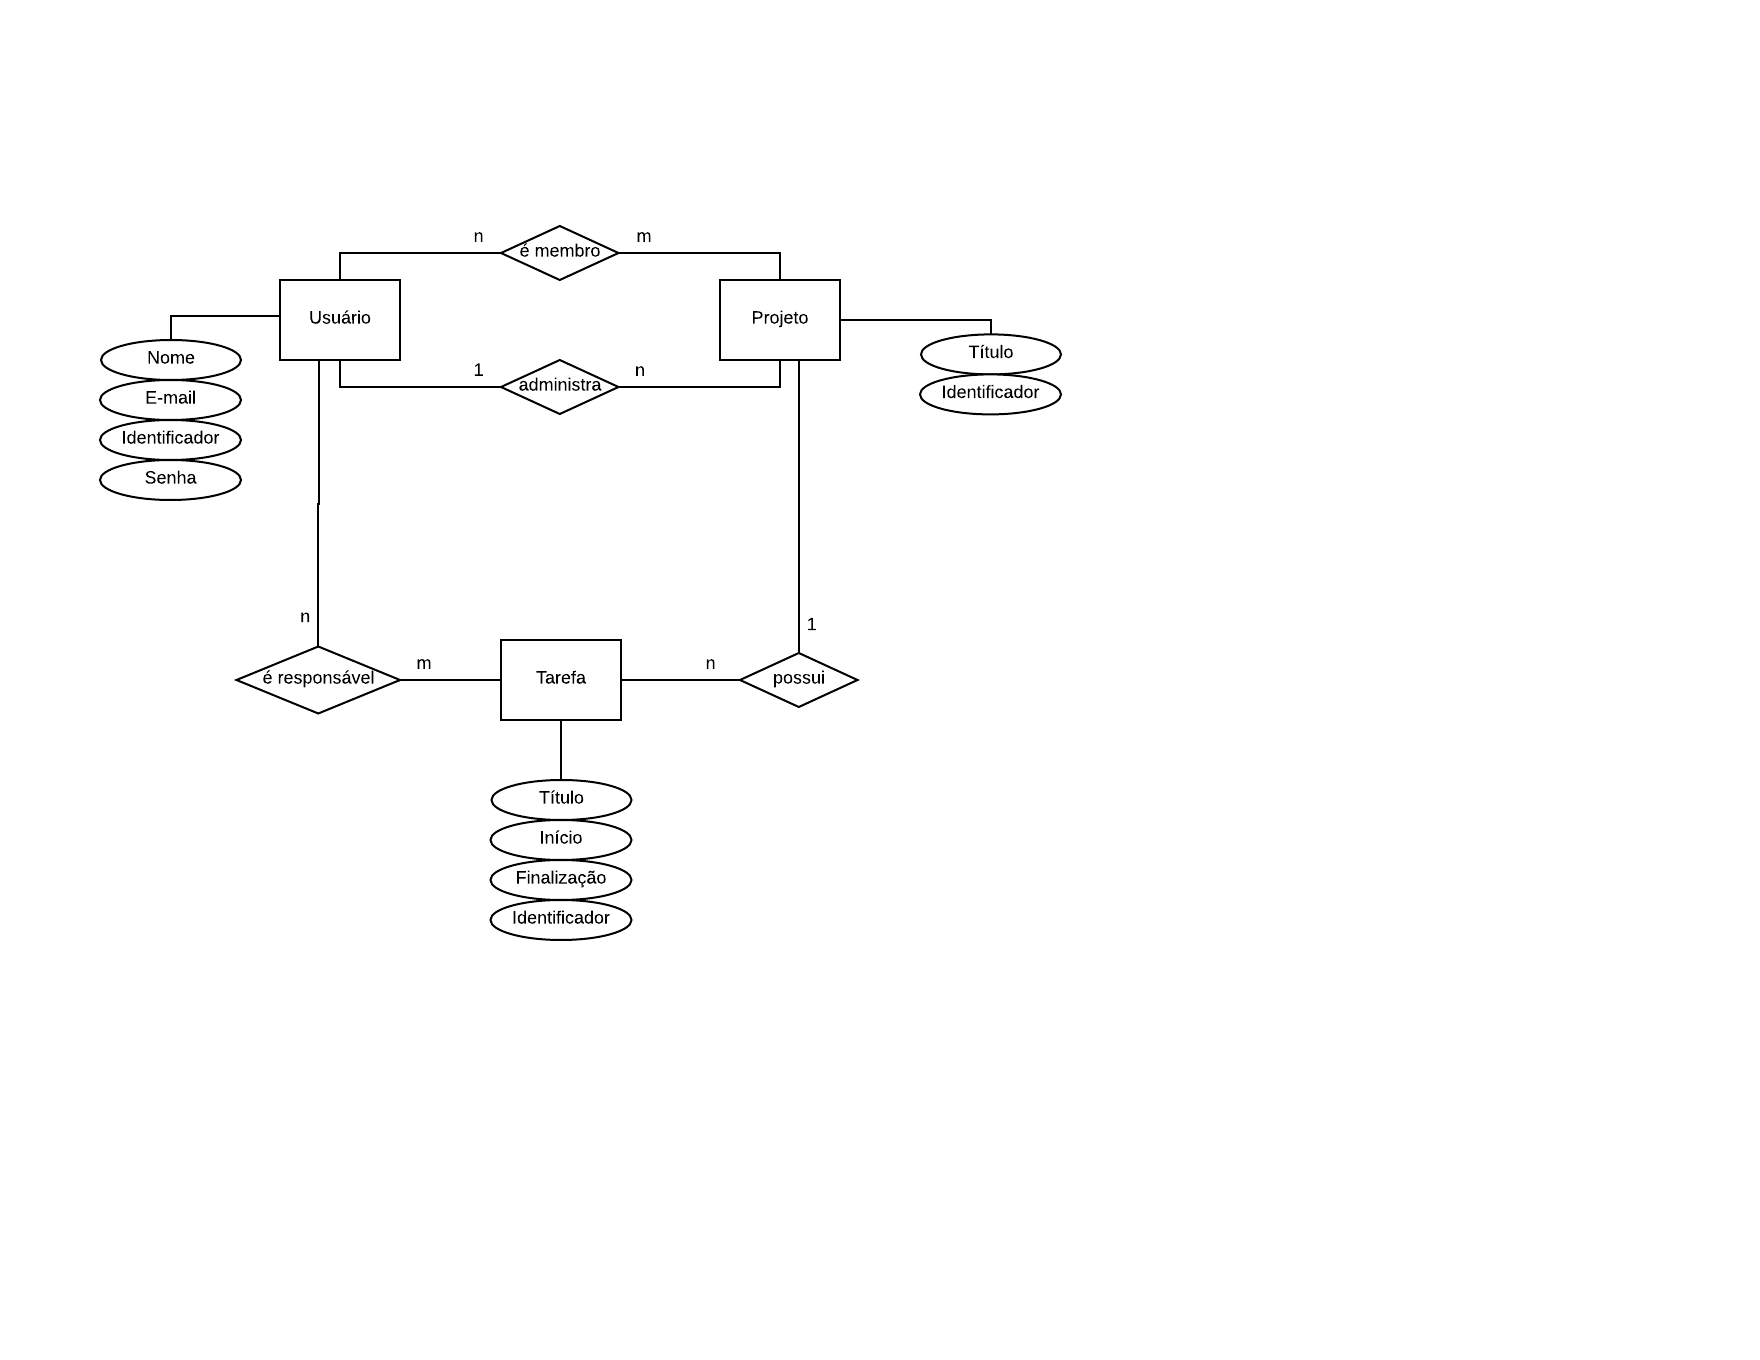
\includegraphics[width=\paperwidth]{diagrama/diagrama.png}
\end{document}


